\documentclass{lni}


\IfFileExists{latin1.sty}{\usepackage{latin1}}{\usepackage{isolatin1}}
\usepackage[utf8]{inputenc}
\usepackage{graphicx}
\usepackage{url}
\usepackage{listings}
\usepackage{nameref}
\graphicspath{{pix/}{}}

\author{Gerhard Gröschl, Miran Mizani\\\{gerhard.groeschl, miran.mizani\}@campus.lmu.de\\\\
Seminar: Trends in Mobilen und Verteilten Systemen \\Wintersemester 2016/2017\\\\
Lehrstuhl für Mobile und Verteilte Systeme\\Institut für Informatik\\Ludwig-Maximilians-Universität München\\\\
Betreuer: Michael T. Beck\\\textit{eingereicht am \today}}
\title{Sicherheitsaspekte bei Deployment virtueller Netzwerkinfrastrukturen}



\begin{document}
\maketitle

\vfill

\begin{abstract}
	Virtualisierung bietet die Möglichkeit Hardware äußert effizient zu nutzen. Serviceprovider müssen die Hardwarebasis für ihre Dienste nicht mehr selbst unterhalten und geben ihre dahingehende Verantwortung an Infrastrukturanbieter weiter. Mobilfunkanbieter sind nicht mehr an dedizierte Hardware gebunden und können die benötigten Funktionen virtualisieren, um nur zwei von vielen Anwendungsfällen zu nennen. Um die Sicherheit dieser Strukturen nicht zu vernachlässigen, arbeiten viele Forscher in diesem Bereich und versuchen effiziente Algorithmen mit integrierter Beachtung der Sicherheitsaspekte zu finden. Diese Arbeit klassifiziert Gefahren, die sich im Kontext der Virtualisierung neu ergeben, und analysiert zwei verschiedene Ansätze zur Vermeidung von späteren Sicherheitsrisiken bereits zum Zeitpunkt der topologischen Planung der virtuellen Netze. 
\end{abstract}


\newpage
\tableofcontents
\newpage

\section{Einleitung}
\label{sec:Einleitung}
%Internet impasse
Ein Konzept dem Internet Impasse mit flexibler Architektur \underline{[WAS IST DAS?]} und Handhabbarkeit zu begegnen, wurde in der Netzwerkvirtualisierung (NV) gefunden. \cite{anderson2005overcoming, bays2012security, fischer2013virtual} Sie basiert auf Knoten- (z.B. Xen) und Linkvirtualisierung \underline{[ANGABE ZU BEIDEM?]} und erlaubt so von der tatsächlichen physischen Hardware und Netzinfrastruktur (NI) beinahe unabhängige logische bzw. virtuelle Netzwerke einzurichten, welche nach außen hin den Anschein physischer Netzwerke erwecken. Die Möglichkeit mehrere virtuelle Maschinen (VMs) pro physischem Host und verschiedene heterogene virtuelle Netzwerke (VNs) auf demselben physischen Substratnetz zu betreiben befördert die Flexibilität der Netzwerkarchitektur und wirkt dem Internet Ossification Problem \cite{anderson2005overcoming} entgegen.

%Vorteile von NV
Die großen Vorteile der NV liegen in der Abstraktion von der eingesetzten Hardware. Das Erstellen, Verändern, Migrieren, Zurücksetzen und Löschen von Maschinen funktioniert genauso einfach wie der Umgang mit Dateien, was eine dynamischere Nutzung des Netzwerkes erlaubt. Virtuelle Maschinen und Netzwerke eigenen sich auch als Testumgebung. Einerseits werden bestehende Systeme im Fehlerfall nicht direkt beeinträchtigt. Andererseits kann neuer Code nun leicht in verschiedenen Umgebungen (Windows, Linux, verschiedengroßer RAM, mit oder ohne Software-Developer-Kits etc.) ohne zusätzliche Hardware getestet und später einfach ausgerollt werden.

NV eröffnet eine Unterteilung des klassischen Internetserviceproviders (ISP) in Service-Provider (SP) und Infrastructure-Provider (InP). Damit gewonnene Freiheiten durch z.B. jeweils unabhängige Technologieentscheidungen[wang2016towards] sind wohl besonders für Unternehmen interessant, die die Hardwarebasis ihrer Dienste nicht mehr selbst unterhalten wollen.\\
Das Anbieten von Software und Hardware als on-demand Ressourcen wird wegen geringeren Wartungsaufwand, verminderte Hardwarekosten durch Koexistenz mehrerer Mieter, aber v.a. wegen Automatisierbarkeit in der Programmierung der Netzwerkumgebung vereinfacht. Dass InPs nicht mehr streng durch Hardware limitiert sind, begünstigt Skalierbarkeit und bspw. lastbedingte Migration von VMs auf andere physische Hosts.\\
Auch für den Kunden bietet NV Vorteile: Unternehmen bezahlen nur noch für diejenigen Ressourcen, die gerade in Anspruch genommen werden. Hochqualitative Hardware kann so zu einem Bruchteil ihres Preises erworben und ungenutzte Hardware reduziert werden. Durch dynamisches Skalieren (z.B. in Zeiten hoher Last) kann die eigene IT-Landschaft mühelos vergrößert werden.

%Ziele von NV
Das Outsourcing von Rechenleistung, Speicher, Inhalten und Netzwerk soll Soft- und Hardware einfacher nutzbar machen und Geschäftsprozesse befördern. Die damit einhergehende Verantwortungsübertragung erfordert eine Anpassung des Risikomanagements und IT-Sicherheitstechnische Arbeiten zur Erhaltung der klassischen C.I.A.-Aspekte. Wegen der gemeinsam genutzten Hardware kommt aus Sicht des Kunden besonders der Isolation und dem Datenschutz eine wichtige Rolle zu.\\
Bekannte Sicherheitsmechanismen wie Verschlüsselung, Firewalls, Intrusion Detection Systeme etc. können zwar auf den virtuellen Komponenten des Netzwerks implementiert werden. Die Sicherheit von Nutzerdaten könne dadurch aber wegen der heterogenen und stark dynamischen Struktur virtueller Umgebungen jedoch nicht garantiert werden. Ferner dürften Vorteile der Netzwerkvirtualisierung durch den zusätzlichen Overhead verloren gehen. \cite{gong2016virtual}\\
Eine mögliche Lösung hierzu ist das Integrieren von Sicherheitsaspekten bereits in die Zuordnung von virtuellen zu physischen Knoten und Links. Dieser Virtual Network Embedding (VNE) Prozess stellt eine der größten Herausforderungen in der Netzwerkvirtualisierung dar. \cite{fischer2013virtual}
Werden virtuelle Netzwerke entsprechend ihrer Sicherheitsanforderungen bereits auf Substratknoten mit hinreichender Schutzfunktion wie beispielsweise Firewall abgebildet, so kann Overhead durch zusätzliche Sicherheitstechnik im laufenden Betrieb des VNs reduziert werden.

[TODO]
Derzeit wird versucht \cite{bays2012security, gong2016virtual, wang2016towards} derartige Probleme bereits im VNE-Algorithmus anzugehen [SVNE Security-aware VNE|security by design]. Nicht allen Problemen bzw. Sicherheitsrisiken kann aber auf diese Weise begegnet werden. %(= Überleitung zur Gliederung und zweiten Kapitel?)


Diese Arbeit soll Gefahren im Kontext virtualisierter Netzwerke klassifizieren und zwei unterschiedliche Ansätze zur Schaffung eines möglichst hohen Sicherheitsniveaus bereits zum Zeitpunkt des VNE-Prozesses analysiert.\\
Dazu wird zuerst das VNE-Problem in Kapitel \ref{sec:VNE-Problem} \textit{\nameref{sec:VNE-Problem}} dargestellt. Kapitel \ref{sec:gefahren} \textit{\nameref{sec:gefahren}} untersucht Sicherheitsanforderungen an virtuelle Netzwerkstrukturen und klassifiziert Sicherheitsrisiken, die sich in deren Kontext ergeben. Zwei Möglichkeiten zur Vermeidung von Gefahren, denen bereits im VNE-Prozess begegnet werden kann, werden im Kapitel \ref{sec:svne} \textit{\nameref{sec:svne}} betrachtet. Nach einer Diskussion in dieser Arbeit offengebliebener Probleme in Kapitel \ref{sec:offenefragen} \textit{\nameref{sec:offenefragen}} wird mit einem Ausblick abgeschlossen.
[KAPITELNAMEN-REFERENZIERUNG NÖTIG? LIEBER OHNE?]



% Die Ausarbeitung zum Seminar soll dem Layout der \textit{GI-Edition Lecture Notes in Informatics (LNI)} entsprechen. Die verwendete Literatur wird in der beiliegenden Datei \verb+literatur.bib+ verwaltet. Eine Referenz kann mittels des \verb+\cite{}+--Kommandos eingefügt werden, z.B.

% \subsection{Hinweise für Abbildungen}
% Abbildungen müssen als \texttt{.pdf}, \texttt{.png}, oder \texttt{.jpg} eingebunden werden. Beispiel:
% \begin{figure}[htb]
%   \begin{center}
%     
\includegraphics[width=1cm]{gilogo.pdf}
%     \caption{\label{logo}Das Logo der GI}
%   \end{center}
% \end{figure}


\section{Das Virtual Network Embedding Problem}
\label{sec:VNE-Problem}
Um den Anforderungen der heutigen Gefahren zu genügen, ist es unumgänglich sämtliche Grundsätze der IT-Sicherheit bereits in die Infrastrukturplanung miteinzubeziehen. Nicht nur, weil das nachträgliche Schließen von Sicherheitslücken und Hinzufügen von Sicherheitskomponenten in finanzieller und zeitlicher Hinsicht zehnmal so teuer ist wie die initiale Beachtung dieser Aspekte, sondern weil die vollständige Sicherheit eines nachgerüsteten Systems kaum gewährleistet werden kann. \cite{Cole} "`Security-by-Design"' ist einer der wichtigsten Begriffe bei der Planung öffentlich zugänglicher Netzwerkstrukturen. Dementsprechend groß ist die Nachfrage nach VNE-Algorithmen, die bereits beim Prozess des Mappings viele Sicherheitsaspekte beachten und abdecken. 
%Die Einteilung von bekannten Gefahren in "`VNE-relevant"' und "`nicht-VNE-relevant"' in Kapitel \ref{subsec:gefahren_vnerelevant} bildet die Grundlage für unsere weiteren Untersuchungen.
Um einen genaueren Einblick in die Problematik von VNE zu gewähren, beginnen wir zunächst mit der Erläuterung des VNE-Problems sowie einem Überblick über die verschiedenen erfolgreichen Strategien bestehender VNE-Algorithmen, welche die Sicherheitsaspekte noch nicht beachten.

Betrachtet man das zugrundeliegende physische System als einen ungerichteten Graphen und extrahiert die vorhandenen Elemente sowie deren Werte, erhält man die Basismenge in welche die virtuellen Strukturen eingebettet werden sollen. Siehe Abbildungen ~\ref{graph1}, ~\ref{graph2} und ~\ref{graph3}.



\begin{figure}[htb]
\begin{center}
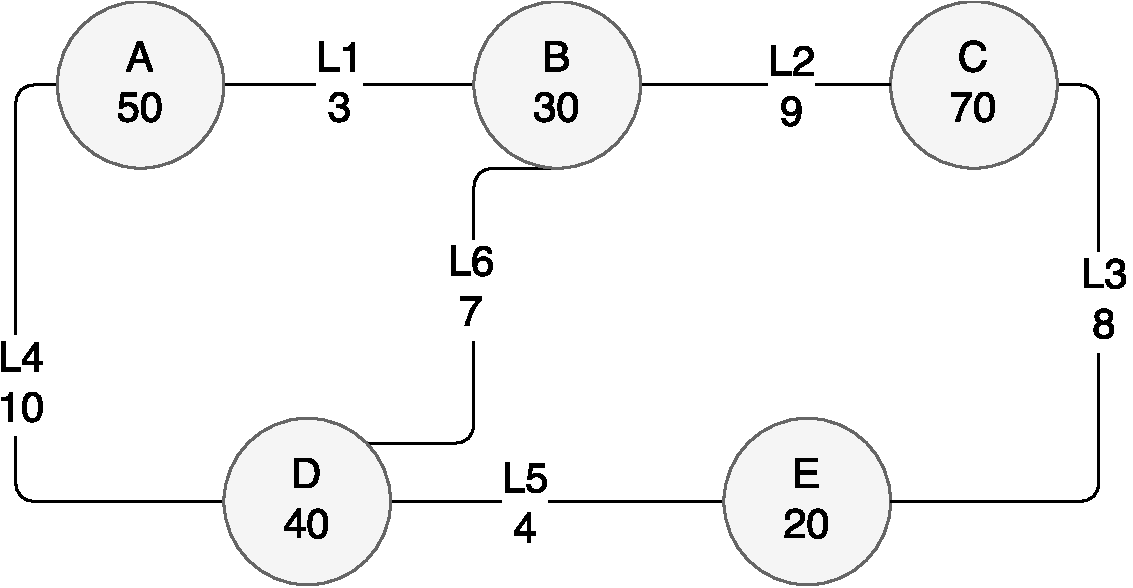
\includegraphics[width=\textwidth]{physical_structure2.pdf}\newline
\caption{\label{graph1}Ungerichteter Graph der physischen Infrastruktur}
\end{center}
\end{figure}

\begin{figure}[htb]
\begin{center}
G\textsuperscript{S} = \{N\textsuperscript{S}, L\textsuperscript{S}\}
\caption{\label{graph2}N steht für die Menge der physischen Knoten, L für die Menge der physischen Links}
\end{center}
\end{figure}

\begin{figure}[htb]
\begin{center}
\hspace{1.0cm}
G\textsuperscript{S} = \{\{
(A\textsuperscript{S},50),(B\textsuperscript{S},30),(C\textsuperscript{S},70),
(D\textsuperscript{S},40),(E\textsuperscript{S},20)\},\newline\{
(L1\textsuperscript{S},3),(L2\textsuperscript{S},9),(L3\textsuperscript{S},8),
(L4\textsuperscript{S},10),(L5\textsuperscript{S},4),(L6\textsuperscript{S},7)\}\}
\caption{\label{graph3} Netz aus Abbildung \ref{graph1} in vereinfachter Mengennotation}
\end{center}
\end{figure}

An dieser Stelle muss darauf verwiesen werden, dass die Mengen in der Realität um einiges komplexer sind. Beispielsweise kann aus der Menge aus Abb. 3 nicht mehr rekonstruiert werden, welcher Link mit welchen Knoten verbunden ist.
\newpage



Ein "`virtual network request"' (in Folge "`VNR"' genannt) kann hierbei ebenfalls als ein ungerichteter Graph gesehen und genauso in eine Menge übersetzt werden. Abbildungen ~\ref{graph4}, ~\ref{graph5} und ~\ref{graph6}

\begin{figure}[htb]
\begin{center}
\hspace{0.8cm}
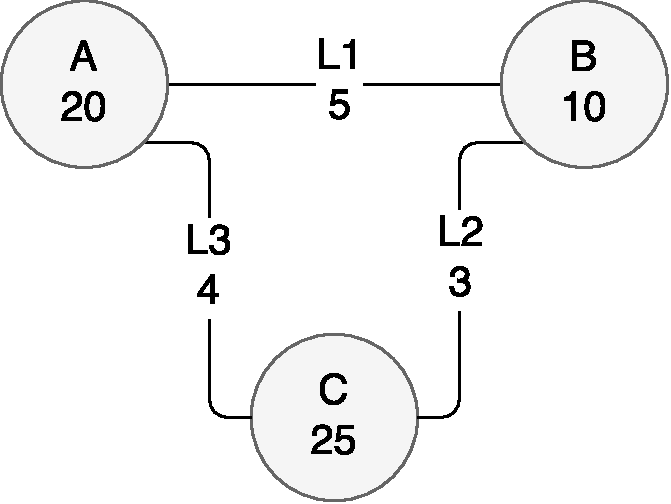
\includegraphics[width=0.7\textwidth]{VNR1.pdf}\newline
\caption{\label{graph4}VNR als ungerichteter Graph}
\end{center}
\end{figure}

\begin{figure}[htb]
\begin{center}
G\textsuperscript{V} = \{N\textsuperscript{V}, L\textsuperscript{V}\}
\caption{\label{graph5}N steht für die Menge der virtuellen Knoten, L für die Menge der virtuellen Links}
\end{center}
\end{figure}

\begin{figure}[htb]
\begin{center}
G\textsuperscript{V} = \{\{
(A\textsuperscript{V},20),(B\textsuperscript{V},10),(C\textsuperscript{V},25)\} , \{
(L1\textsuperscript{V},5),(L2\textsuperscript{V},3),(L3\textsuperscript{V},4)\}\}
\caption{\label{graph6}VNR aus Abbildung 4 in vereinfachter Mengennotation}
\end{center}
\end{figure}


Gesucht ist nun eine Abbildungsfunktion f : G\textsuperscript{V} $\rightarrow$ G\textsuperscript{S}


In der Regel ist es üblich, nicht nur eine einzelne Requests auf ein physisches System abzubilden, sondern gleich mehrere auf einmal. Ebenso wäre es theoretisch möglich, dass ein Infrastruktur-Provider gleich mehrere getrennte unabhängige physische Strukturen betreibt, und somit mittels VNE das beste System für die Abbildung der Menge von VNRs eruieren möchte. Dies könnte beispielsweise der Fall sein, wenn ein Serviceprovider ein VNR mit der Bedingung "`alle Elemente mögen sich am selben Standort befinden, egal an welchem"' in Auftrag gibt, und der Infrastruktur-Provider über mehrere Hardware-Standorte verfügt.
\newline
% Gv=...
Die Attributmenge bei den grundlegenden VNE-Algorithmen beschränkt  sich zumeist auf CPU- und Netzwerk-Leistung. 
Lokalität, GPU-Leistung und RAM-Menge wären einige weitere mögliche Standard-Attribute. Ein großes Problem bei der Berechnung des optimalen Mappings findet sich bei der Berechnungszeit. Die endliche Beschränkung der Knoten- sowie Link-Resourcen und die "`on-line nature"' von VNRs stellen zusätzliche Hindernisse dar. Da selbst Lösungen für einfache Anfragen (geringe Anzahl von Knoten und Links), welche wenige Attribute beinhalten, exponentiellen Rechenaufwand benötigen, steigt der Aufwand sowohl mit der Anzahl der abzubildenden Knoten und Links, als auch mit steigender Attributanzahl dementsprechend. Teilweise gilt das Problem als rechnerisch unlösbar, grundsätzlich aber befinden wir uns im Komplexitätsbereich der NP-Vollständigkeit. \cite{SVNE2} Da die Erhöhung der Attributmenge - wie bereits genannt - grundsätzlich nicht positiv zur Laufzeit der existierenden Algorithmen beiträgt, werden wir den Komplexitätsbereich beim Hinzufügen von Sicherheitsanforderungen nicht verlassen. Dennoch gibt es Möglichkeiten, die den Rechenaufwand reduzieren können. Da neben solchen Performace- auch Sicherheitsapekte in den VNE-Algorithmus eingehen sollen, werden nun bekannte Risiken virtueller Netze betrachtet.



\section{Sicherheitsaspekte virtueller Netzinfrastrukturen}
\label{sec:gefahren}
Das Folgende Kapitel klassifiziert bekannte Sicherheitsrisiken in virtuellen Netzwerken. Anschließend wird untersucht, welche von ihnen bereits im VNE-Prozess begegnet werden kann.


%\subsection{(Sicherheits-)Anforderungen an virtualisierte Umgebungen}
%\label{subsec:gefahren_anforderungen}
%Dummytext. :)


\subsection{Neue Verwundbarkeiten in virtualisierten Umgebungen}
\label{subsec:gefahren_virt}
Wie in der Einleitung dieser Arbeit angedeutet bietet Netzwerkvirtualisierung einige Vorteile gegenüber bisherigen Netzarchitekturen. Durch die Einführung einer weiteren Schicht zwischen Hardware und Anwendungssoftware (,,Ebene virtueller Netze'' in Abbildung \ref{fig:gefahren_dreiEbenenDerVirtualisierung}) und dem Hosten verschiedener virtueller Netzwerke auf einem gemeinsamen Substratnetz tun sich aber auch verschiedene -- im Gegensatz zu herkömmlichen, nicht-virtualisierten Architekturen -- neue Verwundbarkeiten auf. \cite{gong2016virtual, natarajansecurity, wu2010network, garfinkel2005virtual, dahbur2011survey} haben bereits einige Sicherheitsrisiken analysiert, welche im Folgenden klassifiziert und ergänzt werden.

\begin{figure}[htb]
	\begin{center}
		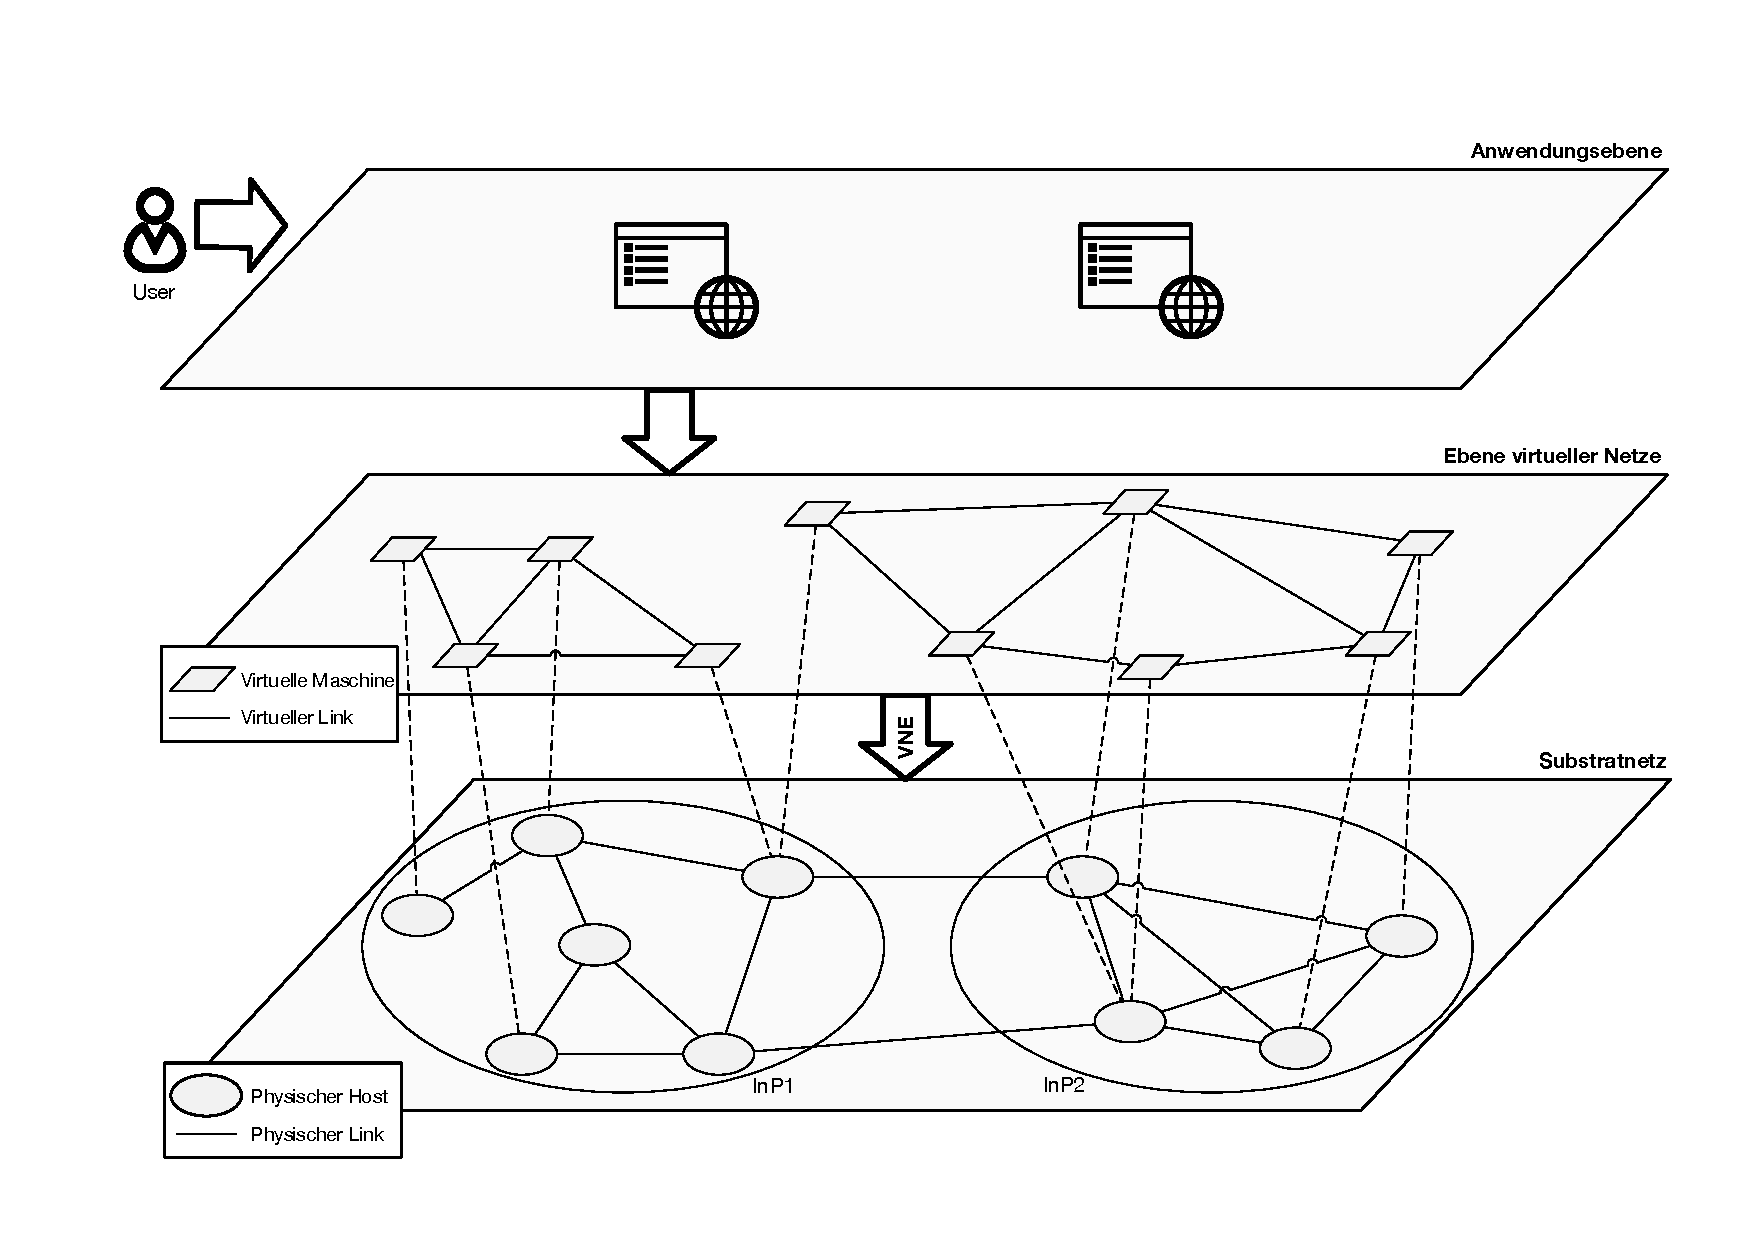
\includegraphics[width=\textwidth]{gefahren_dreiEbenenDerVirtualisierung.pdf}
		\caption{\label{fig:gefahren_dreiEbenenDerVirtualisierung} Drei-Schichtenarchitektur der Netzwerkvirtualisierung. \newline
		Das Substratnetz zweier InP hostet zwei virtuelle Netze.}
	\end{center}
\end{figure}

Dummytext. :)


\subsubsection*{Technischer Art}
\label{subsubsec:gefahren_virt_technisch}
Dummytext. :)

\paragraph{von NI}
\label{parag:vonNI}
bla bla

\paragraph{von VN/VM}
\label{parag:vonVN}
bla bla

\paragraph{von User}
\label{parag:vonUser}
bla bla


\subsubsection*{Organisatorischer Art}
\label{subsubsec:gefahren_virt_organisatorisch}
Dummytext. :)

\subsubsection*{Rechtlicher Art}
\label{subsubsec:gefahren_virt_rechtlich}
Dummytext. :)




\subsection{VNE-relevante Gefahren}
\label{subsec:gefahren_vnerelevant}	
Das Integrieren von Sicherheitsfaktoren in den VNE-Prozess verspricht eine Verringerung der Risiken für alle Interessensgruppen ohne zusätzlichen Overhead im laufenden Betrieb der VNs. Nicht allen Sicherheitsrisiken kann jedoch allein im VNE-Prozess begegnet werden. \cite{fischer2013virtual, wang2016towards} 
Dieses Kapitel untersucht, welche der im Kapitel \ref{subsec:gefahren_virt} aufgeführten Risiken bereits im VNE-Prozess adressiert, d.h. durch geeignete Wahl der Abbildung von virtuellen auf physische Knoten verringert werden können. Solche Gefahren werden in dieser Arbeit als „VNE-relevant“ bezeichnet. 

Da Risiken innerhalb der Anwendungsebene oder des Substratnetzes nur herkömmliche und keine durch Virtualisierung neu hinzukommende Verwundbarkeiten beinhalten, können sie nicht VNE-relevant sein. Herkömmlichen Gefahren, die unabhängig von Virtualisierung sind, kann durch den VNE-Prozess ebenfalls nicht begegnet werden.\\
Risiken, die mit dem User bzw. der Anwendungsebene (vgl. Abbildung \ref{fig:gefahren_dreiEbenenDerVirtualisierung}) assoziiert sind, können nicht VNE-relevant sein, da sie unabhängig von der Wahl der Abbildung von VN bzw. VM auf physischen Host bestehen bleiben. Auch Userangriffe während des Migrationsprozesses sind nicht VNE-relevant, da sie nicht durch die Wahl der Abbildung auf physische Hosts verhindert werden können. Einzig gegen (D)DoS-Angriffe auf Anwendungsebene z.B. über HTTP kann im VNE-Mapping begegnet werden, indem z.B. das entsprechende VN auf Hosts mit entsprechender (D)DoS-Erkennung bzw. Filterung abgebildet wird.

Somit bleiben Gefahren der Kategorien I.2 (von NI ausgehend gegen VN/VM), II.1 (von VN/VM ausgehend gegen NI) und II.2 (von VN/VM ausgehend gegen VN/VM) aus Abbildung \ref{fig:gefahren_klassifizierung} zu untersuchen.\\
Da dem VNE-Prozess nur beschränkt Informationen zur Verfügung stehen, welche Operationen eine VM später ausführen wird und ob diese auf Kompromittierung ihres physischen Host abzielen, werden Gefahren aus Kategorie II.1 hier als nicht VNE-relevant angesehen. 
Risiken der Kategorie I.2 wie Sniffing, Spoofing der Monitoring der VM-Aktivität durch den physischen Host lassen sich durch Abbildung auf „vertrauenswürdige“ Hosts adressieren, die der VM keinen Schaden zufügen. Unabhängig davon wie „Vertrauenswürdigkeit“ festgelegt oder erkannt wird, sind solche Gefahren VNE-relevant.\\
Verwundbarkeiten, die in Kapitel \ref{subsubsec:gefahren_virt_technisch} unter II.2 aufgeführt wurden, basieren auf einer Verletzung der Isolation der VNs bzw. VMs über Schwachstellen in gemeinsam genutzten Ressourcen. Durch Abbildung auf getrennte physische Hosts können solche Risiken umgangen und somit als VNE-relevant bezeichnet werden. Bedingungen zum Kohosting gewisser VNs lassen sich in den VNE-Algorithmus integrieren. 

Da Bedrohungen der Vertraulichkeit und Integrität auf Isolationsverletzungen beruhen, sind solche Risiken organisatorischer Art VNE-relevant. Snapshotproblem und Schwierigkeiten im Patchmanagement können durch den VNE-Prozess jedoch nicht adressiert werden.
Regeln zur Abbildung von VNs bzw. VMs in andere Länder können in den VNE-Algorithmus aufgenommen werden.

%~\newline
%[ZUSAMMENFASSUNG]
%
%Klassifizierung abgeschlossen. ...
%
%Auf welche Weise VNE-relevanten Risiken im VNE-Algorithmus begegnet werden kann, wird im folgenden Kapitel untersucht.
%
%[ÜBERLEITUNG]


\section{Vermeidung von Gefahren via Secure VNE (SVNE)}
\label{sec:svne}
Da wir nun einen Überblick zu VNE sowie den bestehenden Gefahren gegeben haben, widmen wir uns nun zwei verschiedenen SVNE-Lösungsansätzen. Der Detailgrad wurde so gewählt, dass man einen guten Einblick in die Arbeitsweise der Ansätze bekommt und die Problematik der zusätzlichen Last der Sicherheitsaspekte erkennt.

\subsection{Ansatz 1: Strikte Trennung und Preprocessing}
\label{subsec:ansatz1}

Hierbei beschäftigen wir uns mit dem Lösungsansatz aus \cite{wang2016towards}. 
Das Hauptaugenmerk bezüglich der Sicherheitsaspekte legen Wang et. al. auf Traffic-Verschlüsselung und die Separierung von VMs unterschiedlicher Trust-Levels. Die drei folgenden strukturellen Aspekte werden betrachtet und in dementsprechende Levels eingeteilt.
\begin{itemize}
\item Netze:\newline
Ein VNR wird als Netzwerk betrachtet und seinem Level entsprechend isoliert. "`High"' fordert und beansprucht ein gesamtes Netz bzw. Subnetz der physischen Infrastruktur für sich. Hiermit soll die Wahrscheinlichkeit für DOS-Angriffe oder ähnliche vermindert werden, da "`Mehr-Parteien-Netzwerke"' die Hauptschwachstellen für solche Angriffe darstellen. \cite{DOS} Auch Sniffing durch kompromittierte Hosts im selben Netz wird durch diese Maßahme verhindert. Während "`high"' Resourcenteilung somit komplett verweigert, lässt der Level "`medium"' zumindest ein gemeinsam genutztes Netz für VNRs vom selben Eigentümer zu.

\item Knoten:\newline
Die einzelnen virtuellen Knoten eines VNR stellen Isolierungsanforderungen an die physischen Knoten. Wie auch beim Netzaspekt, werden die Levels "`high", "`medium"' und "`none"' definiert und umgesetzt. "`high"' fordert die alleinige Existenz eines VNR-Knotens, "`medium"' lässt VNR-Knoten vom selben Eigentümer auf ein und demselben physischen Knoten zu. Durch diesen Plan sollen Angriffe von VM zu VM über gemeinsam genutzte Resourcen unterbunden werden. Zusätzlich wird das Risiko eines Angriffs vom physischen Host verringert, da der Angriffsvektor "`VM zu physischem Host"' eliminiert wird.

\item Links:\newline
End-to-End(E2E), Point-to-Point(P2P) und "`none"' sind die hier wählbaren Levels. Während E2E nur an den Endpunkten Verschlüsselungskapazitäten zu Verfügung stellen muss, benötigt P2P diese Kapazitäten an allen Hops des abgebildeten Links. Die heutzutage sehr gängigen man-in-the-middle Angriffe sollen dadurch wesentlich erschwert werden. 
\end{itemize}
VNRs werden nun, wie in Kapitel 2 bereits gezeigt, in ungerichtete Graphen mit Standardanforderungen transformiert. Zusätzlich werden hier auch noch Sicherheitsanforderungen integriert. Siehe Abbildung ~\ref{graph7}.\newline

\begin{figure}[htb]
\begin{center}
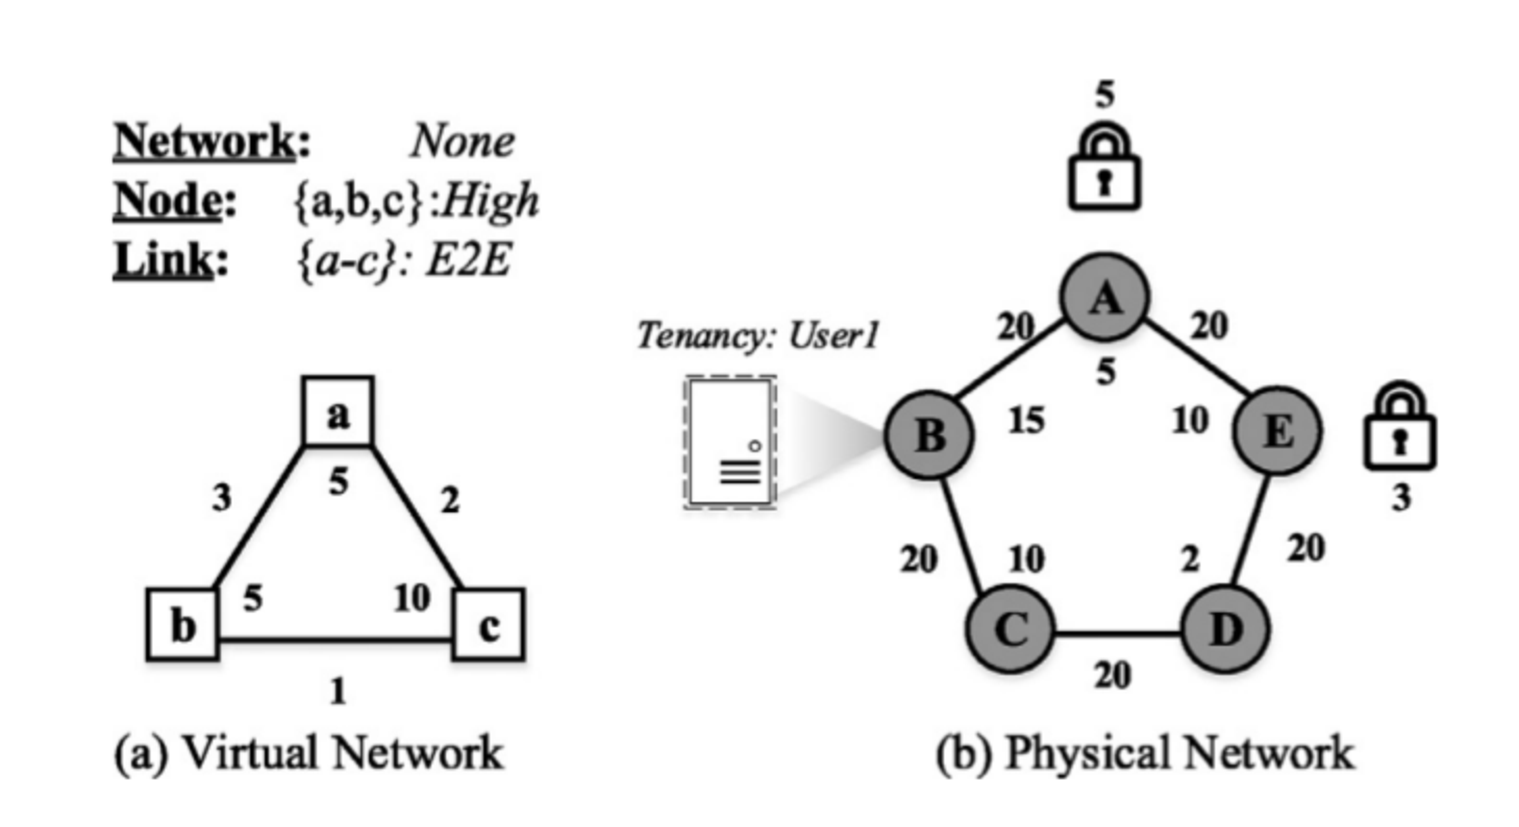
\includegraphics[width=0.8\textwidth]{SVNR.pdf}\newline
\caption{\label{graph7}VNR und physisches System mit Sicherheitsmerkmalen \cite{wang2016towards}}
\end{center}
\end{figure}

Nun wird ein vier-stufiges Pre-Processing durchgeführt, um die Berechnung der optimalen Abbildung der VNRs zu vereinfachen. Hierbei werden als ersten die Standardanforderungen der virtuellen Knoten mit den zu Verfügung stehenden Kapazitäten der physischen Knoten verglichen. Sollten physische Knoten bestimmte Anforderungen nicht erfüllen, werden sie aus der Berechnung ausgeschlossen. Der zweite Schritt ist den Netzen gewidmet. Sollte ein physischer Knoten, welcher den Anforderungen des Netzes nicht genügt sich in einem Kandidaten-Netzwerk befinden, wird das Subnetz aus den Berechnungen ausgeschlossen. Im dritten Schritt werden die Sicherheitsanforderungen der einzelnen Knoten betrachtet und nicht entsprechende physischen Knoten werden abermals entfernt. Der letzte Schritt widmet sich den Sicherheitsanforderungen aus der Links und streicht Links aus den weiteren Berechnungen, welche den Verschlüsselungsanforderungen der virtuellen Links nicht genüge tun. Siehe Abbildung~\ref{graph8}.

\begin{figure}[htb]
\begin{center}
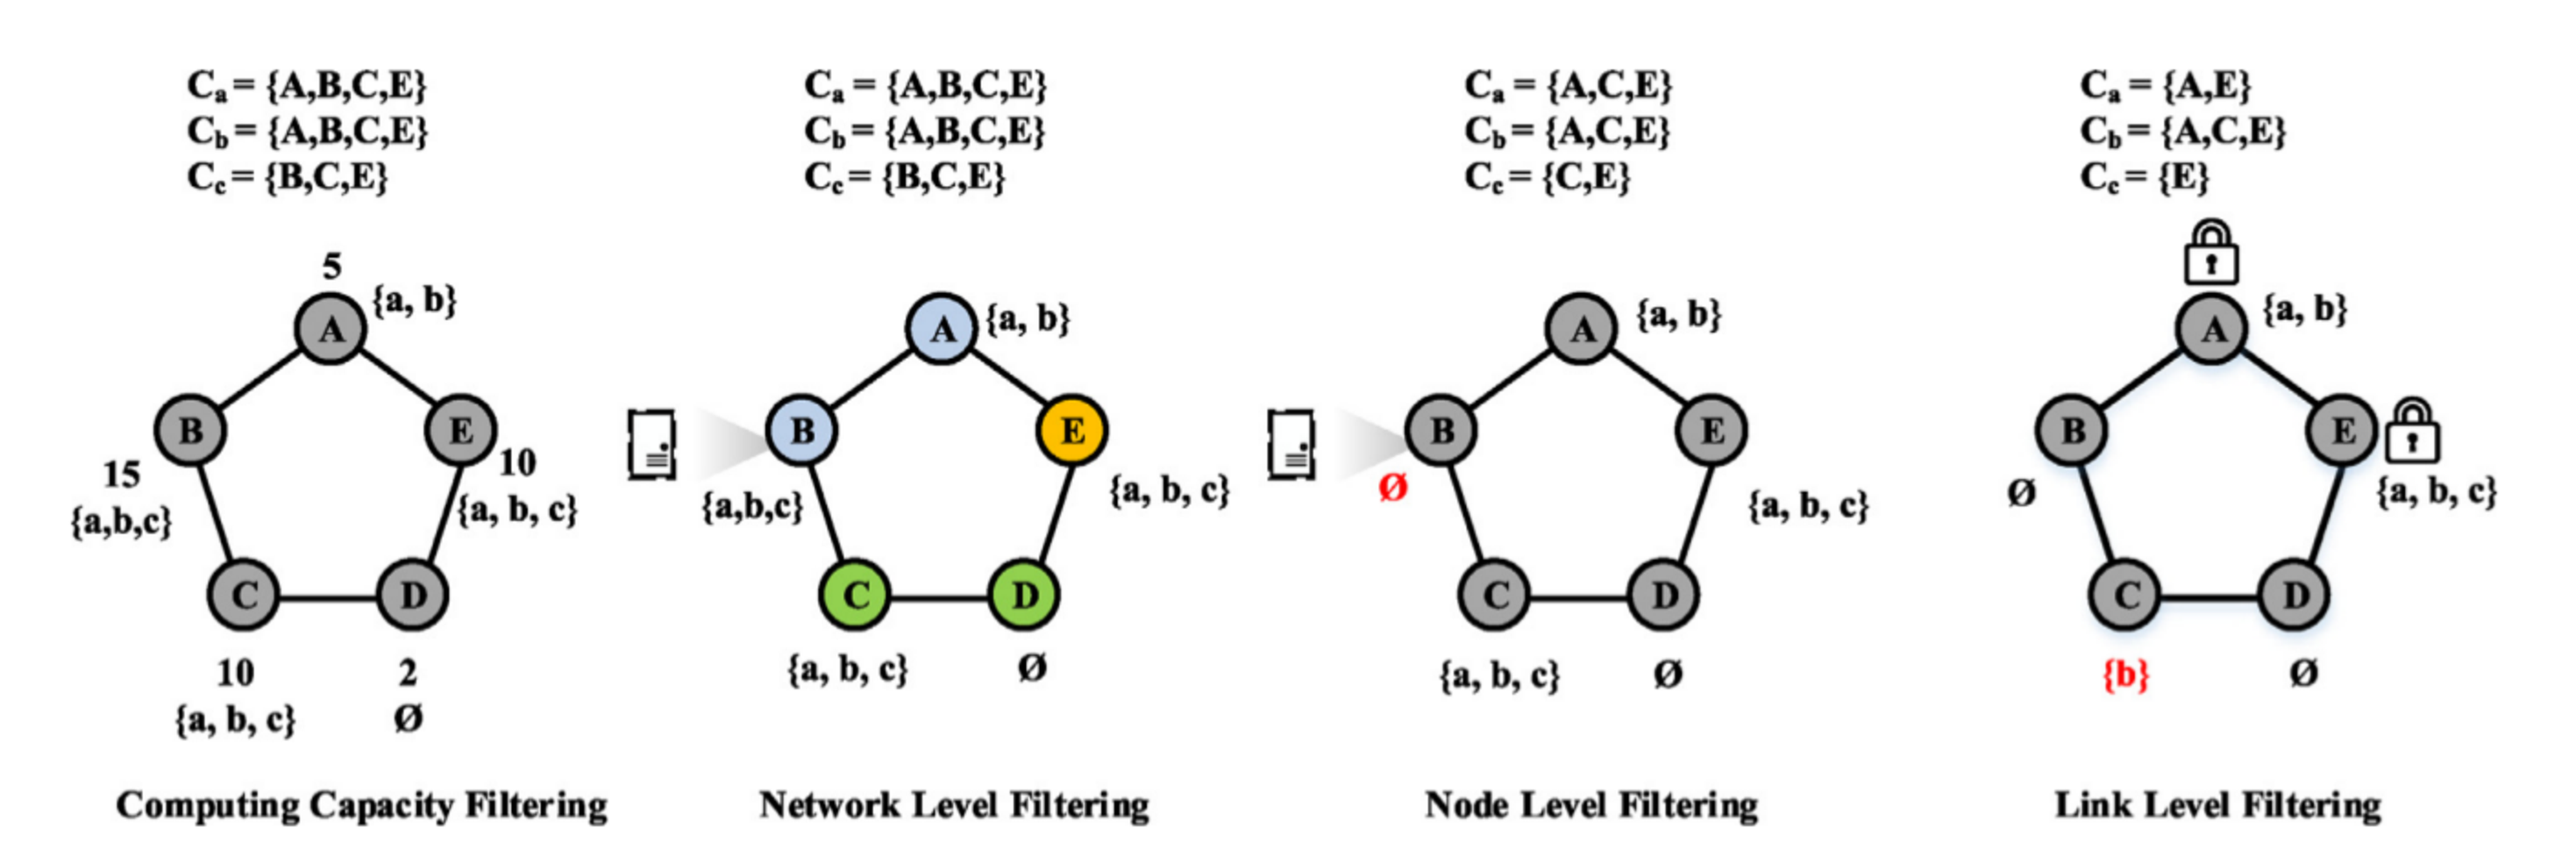
\includegraphics[width=0.75\textwidth]{pre-processing.pdf}\newline
\caption{\label{graph8}4-stufiges Pre-Processing\cite{wang2016towards}}
\end{center}
\end{figure}

Mit den aus dem Pre-Processing gewonnen Information bildet man nun einen Hilfsgraphen, welcher die übrig gebliebenen Möglichkeiten der Einbettung zeigt. Siehe Abbildung~\ref{graph9}.

\begin{figure}[htb]
\begin{center}
	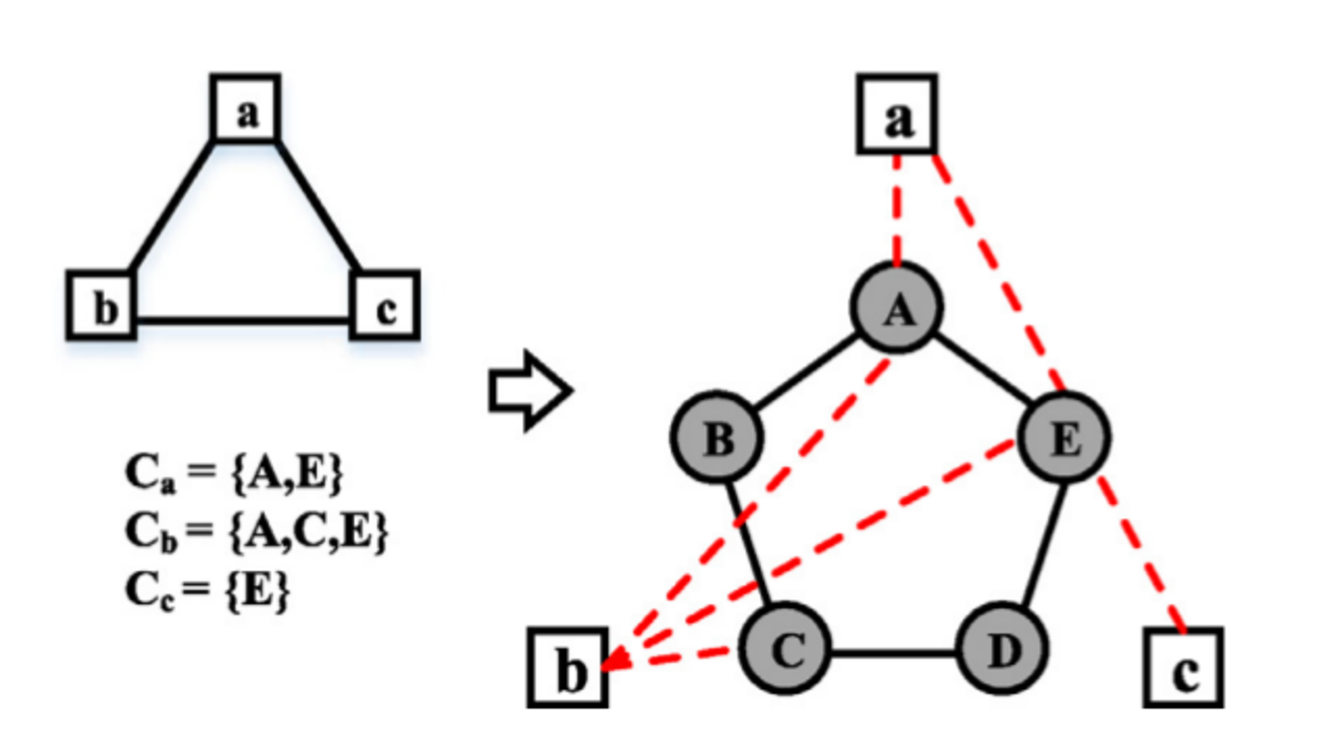
\includegraphics[width=0.6\textwidth]{auxgraph.pdf}\newline 
	\caption{\label{graph9}Hilfsgraph\cite{wang2016towards}}
\end{center}
\end{figure}

Dieses Pre-Processing reduziert das SVNE-Problem auf ein "`multi-commodity-flow"' Problem. \cite{MCF}
Im weiteren Vorgehen werden nun zwei Fälle unterschieden. "`Path-splitting", im weiteren SVNE-PS und "`no-path-splitting"', im weitern SVNE-NPS, sind zusätzliche Sicherheitsvorgaben, welche im Vorfeld definiert werden müssen, um die Wahl des Algorithmus zu ermöglichen. Sollte SVNE-PS gewählt werden, beziehen sich die Gleichungen nur auf die Erfüllung der geforderten Attribute.
Sollte SVNE-NPS gewählt werden, werden die für Link-Abbildungen verantwortlichen Gleichungen ersetzt.\newline

Die Berechnungen wurden unter Verwendung von CPLEX und durch k-shortest-path anhand aller abzubildenden Elemente limitiert. \cite{CPLEX}
Für die Testumgebungen wurden zufällig erzeugte VNRs mit 2 bis 10 Knoten und halbsovielen Links erzeugt. Auch die Rechenkapazität wie Bandbreite wurden durch Zufallsgeneratoren mit Werten im Bereich von 1 bis 10 gewählt und verteilt. Die Anzahl der VNRs beträgt einer Poisson-Verteilung nach einen Durchschnitt von 4 VNR pro 100 Zeiteinheiten, mit einer jeweiligen durchschnittlichen Einsatzzeit von 1000 Zeiteinheiten.

Die zugrundeliegenden physischen Netze wurden ebenfalls zufällig erzeugt und beinhalteten 10 bis 50 Knoten, sowie halbsoviele Links. Die Rechen- sowie Bandbreiten-Kapazitäten wurden gleichmäßig verteilt und enthielten Werte zwischen 1 und 50. Die Verschlüsselungskapazitäten der Knoten  wurde über die gesamte Testreihe ebenfalls gleich"-mäßig verteilt.

Die folgende Statisk zeigt einen Durchschnittsvergleich zwischen dem, als Standard ge"-wählten, VNE-Algorithmus und den beiden SVNE-Varianten PS und NPS. \cite{Std} Dazu sei gesagt dass sämtliche Algorithmen ihre Berechnungen anhand des Hilfsgraphen durchgeführt haben und durch k=3 bzw. k=4 limitiert wurden. Abbildung ~\ref{graph10} \newline

\begin{figure}[htb]
\begin{center}
	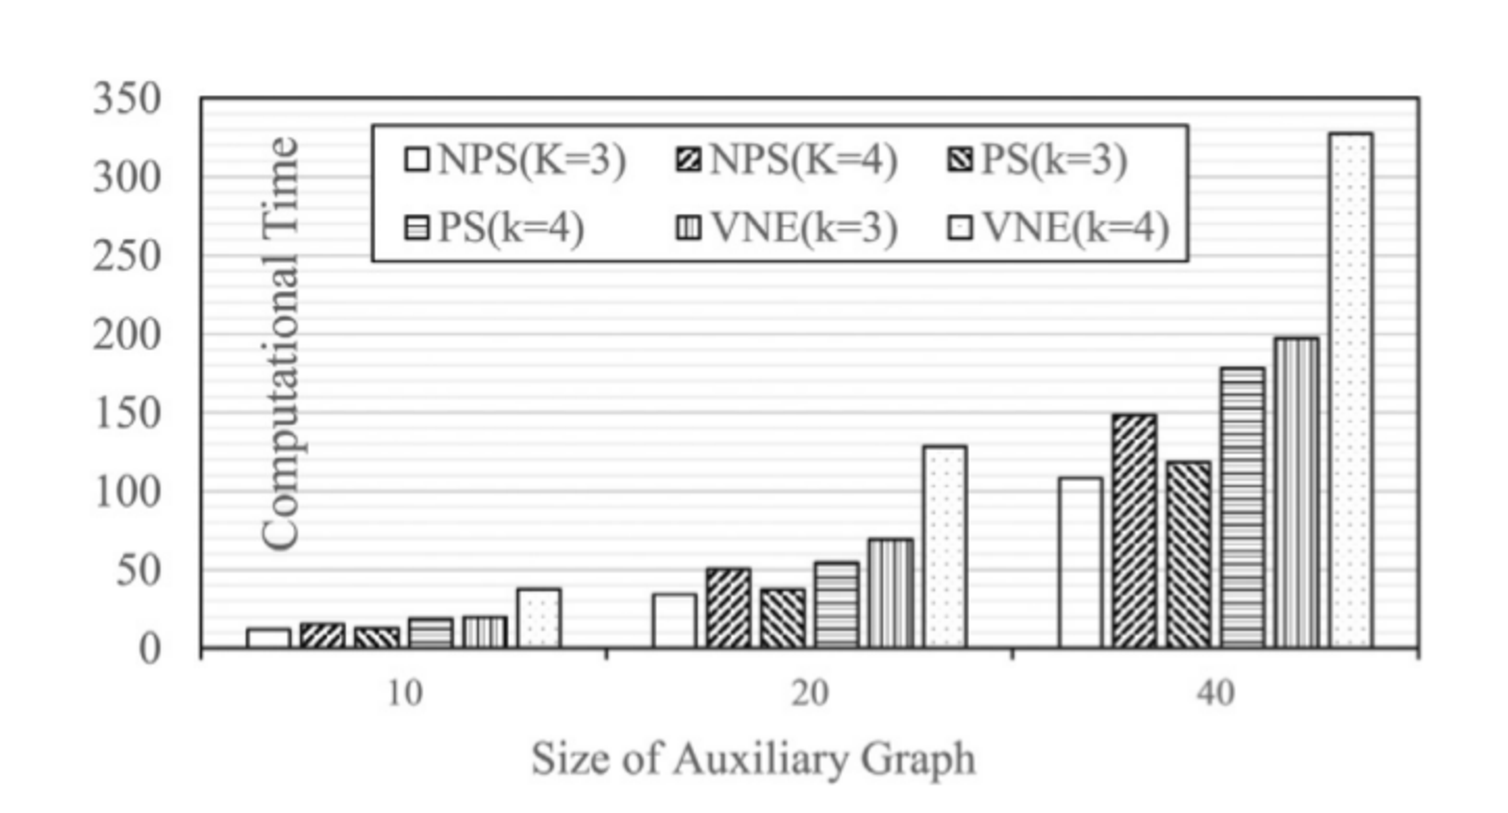
\includegraphics[width=0.8\textwidth]{statistic.pdf}\newline
	\caption{\label{graph10} Evaluationsergebnis \cite{wang2016towards}}
\end{center}
\end{figure}

Man sieht  hier einen deutlichen Zeitvorsprung von PS und NPS gegenüber dem Standard-Algorithmus, was auf eine Optimierung der Algorithmen auf den Outnput des Pre-Pro"-cessings schließen lässt. Da hier jedoch auch der Standard-Algorithmus vom Pre-Processing profitiert, wäre ein Vergleich, welcher die Dauer des Pre-Processings mit aufnimmt und den Standard-Algorithmus ohne Pre-Processing arbeiten ließe, anschaulicher und aussagekräftiger.
Dennoch ist ein Punkt durchaus überraschend und bemerkenswert: Der Standard-Algorithmus benötigt deutlich länger, obwohl er keine Sicherheitsaspekte mitbeurteilt, im Gegenzug zu seinen Kontrahenten.

In welchem Komplexitätsbereich sich das Pre-Processing befindet wird hier leider nicht erwähnt.


\subsection{Ansatz 2: Sicherheitsvektoren und doppelte Berechnung}
\label{subsec:ansatz2}

Im zweiten Ansatz widmen wir uns dem Modell aus \cite{algo2}. Dieser Ansatz arbeitet mit abstrakten Sicherheitslevels. Im Folgenden werden Skalare hierfür verwendet, was allerdings nicht zwingend so vorgesehen ist. Stattdessen wäre eine Verwendung komplexerer Sicherheitsvektoren möglich, welche bei weitem detailliertere Sicherheitsmerkmale  beschreiben könnten. Des weiteren verfügt jeder physische wie auch virtuelle Knoten über zwei Sicherheitswerte: Anforderungslevel und (eigenes) Sicherheitslevel. Der Anforderungslevel definiert das Minimum-Level des Gegenübers, der Sicherheitslevel definiert die eigenen gewünschten Sicherheitsmerkmale. Virtuelle Links verfügen über Anforderungslevels, physische Links nur über Sicherheitslevels. Die vorausgesetzten Basisanforderungen, welchen alle VNRs unterliegen, beschränken sich auf 4 Regeln, welche mittels der zuvor genannten Merkmale umgesetzt werden:
\begin{itemize}
\item Physische Knoten sollten Sicherheitslevels garantieren, 
   die größergleich sind, als die Anforderungen der darauf abzubildenden
   virtuellen Knoten.

\item Die Sicherheitslevels des virtuellen Knoten sollten größergleich sein, 
   als das Anforderungslevels der entsprechenden physischen Knoten.

\item Alle virtuellen Knoten, welche auf den selben physischen Knoten
   abgebildet werden, sollten über einen ausreichenden und gleichmäßigen Sicherheitslevel
   verfügen. 

\item Der Anforderungslevel des virtuellen Links sollte stets kleinergleich
   sein, als das Sicherheitslevel des physischen Links.
\end{itemize}

Der erste und zweite Punkt dienen der Risikominimierung zwischen physischen und virtuellen Hosts in beide Richtungen. Der dritte Punkt stellt sicher, dass keine zu schwach gesicherten VMs zusammen mit stark gesicherten VMs abgebildet werden und somit keine offentsichtlichen Schwachstellen den physichen Knoten samt seiner vituellen Hosts gefährden. Punkt 4 sorgt für ausreichende Sicherheitmechanismen der physischen Links.

\begin{figure}[htb]
\begin{center}
	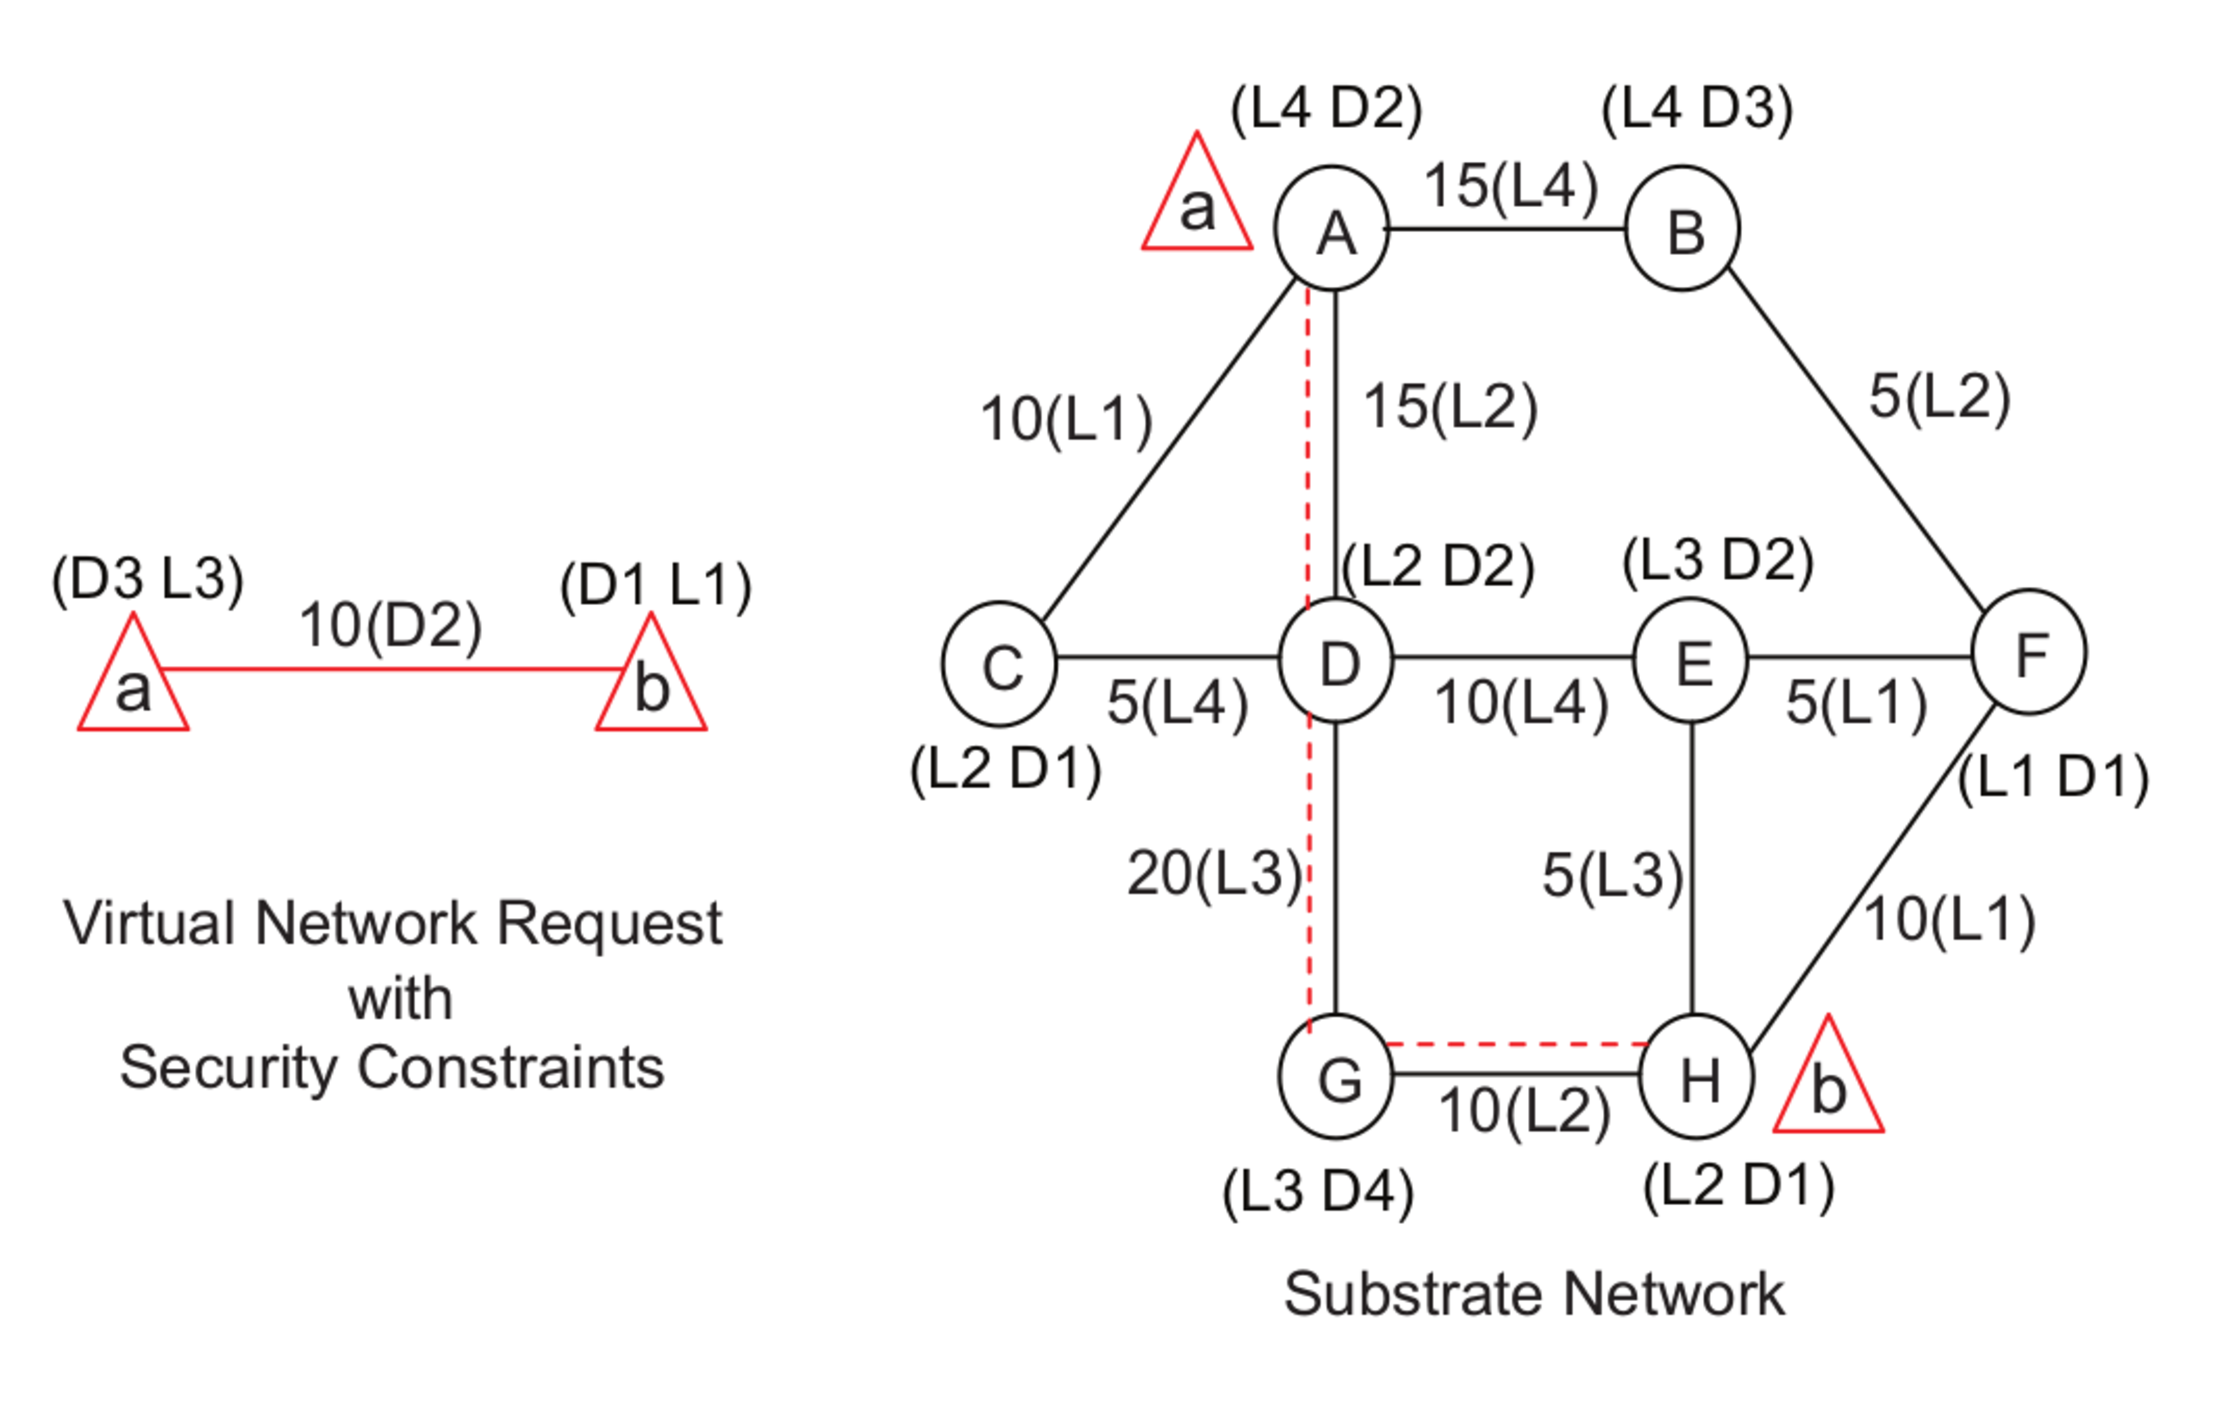
\includegraphics[width=0.8\textwidth]{algo2graph.pdf}\newline
	\caption{\label{graph11} VNR und physisches System mit Sicherheitsmerkmalen\cite{algo2}}
\end{center}
\end{figure}

Wie man in Abbildung~\ref{graph11} sieht, werden auch bei diesem Modell VNRs und physische Netze in ungerichtete Graphen transformiert. Die in Klammern gestellten Parameter beschreiben Anforderungslevel(D) und Sicherheitslevel(L). Die hier durchgeführte Abbildung berücksichtigt nicht nur die Sicherheitsanforderungen aller Parteien unter Berücksichtigung der Basisanforderungen, sondern achtet zusätzlich noch auf Kostenminimierung. Insgesamt existieren drei Abbildungsmöglichkeiten, die gewählte ist jedoch die günstigste, unter dem Aspekt keine Sicherheitsresourcen zu verschwenden. Dieser VNR hätte auch auf EDGH abgebildet werden können, wobei der Link ED über einen Sicherheitslevel verfügt, welcher höher als nötig ist. Würde dies nicht beachtet werden, könnte es zu unnötigen Engpässen bei der Behandlung von VNRs mit höheren Anforderungslevels kommen. Um ein solches Verhalten zu erreichen, wurden zusätzlich Kosten- und Nutzen-Funktionen in die Berechnung integriert.

Das Außergewöhnliche bei diesem Ansatz ist die Verwendung zweier unterschiedlicher Algorithmen, welche sich gegenseitig ergänzen: uSAV und cSAV.
\begin{itemize}
	\item uSAV \newline
	uSAV, der unkooridinierte zwei-Phasen-Algorithmus, behandelt Knoten- und Link-Abbildungen getrennt voneinander. Zuerst werden die Knoten abgebildet, danach erst die Links. Dementsprechend liegt die Schwäche von uSAV in der Abbildung von non-splittable-links. uSAV ist ein terminierender Algorithmus, welcher die Abbildung der Knoten priorisiert und dahingehend ein sehr gutes Ergebnis mit wenig Aufwand erzielt. Jedoch kann es, durch die Priorisierung der Knoten, zu hohen Kosten bei der Link-Abbildung kommen.

	\item cSAV \newline
	cSAV, der koordinierte Algorithmus, behandelt Knoten und Links gemeinsam, und kann zur Optimierung, des bereits von uSAV gelieferten Ergebnisses verwendet werden. cSAV liefert zwar bessere Ergebnisse als uSAV, benötigt aber auch mehr Zeit. Hier muss Zeitaufwand mit gelieferter Leistung abgewogen werden.

\end{itemize} 

Der Author schlägt für ideale Ergebnisse eine kombinierte bzw. parallele Benutzung der beider Algorithmen vor. 

cSAV als auch uSAV nutzen die selben Heuristiken. Diese Heuristiken erstellen, unter Berücksichtigung der einzelnen Request-Details, ein Ranking der physischen Knoten und helfen den Algorithmen bei der Wahl der besten Abbildung. Je mehr CPU- und Netz-Kapazitäten ein Knoten übrig hat, desto höher steigt er in der Rangliste. Die verfügbaren Sicherheitsmerkmale des Knotens erhöhen die Platzierung des Knotens nur bedingt, da auch hier keine Sicherheitsresourcen verschwendet werden sollen. Stimmt der Sicherheitslevel mit dem Anforderungslevel des VNR exakt überein, erhält der Knoten die maximalen Punkte seitens des Sicherheitskriteriums. Auch die vom Knoten ausgehenden Links werden analysiert und in die Berechnung miteinbezogen. Um die Rechenzeit der iterativen Heuristikberechnung im Zaum zu halten, wird die Anzahl der Durchläufe mittels der MaxIte-Variable begrenzt. 



Die Testumgebung dieses Ansatzes wurde mittels GT-ITM-Tool erstellt. \cite{GT-ITM-Tool} 

Die physischen Netze wurden in der Größenordnung eines mittleres ISP angesetzt, und betrugen 100 Knoten und 500 Links. Die Bandbreite und Rechenkapazität wurden, wie auch im vorherigen Ansatz, gleichmäßig verteilt und betrugen Werte zwischen 50 und 100. Die abstrakten Sicherheitslevels der physischen Elemente wurden zwischen 0 und 4 gleichmäßig verteilt. Die Anforderungslevels wurden ebenfalls aus dem Bereich 0-4 gewählt, und so verteilt, dass kein physisches Element ein höheres Anforderungslevel als Sicherheitslevel besitzt.

Die VNRs beinhalteten 2 bis 20 Knoten sowie halbsoviele Links. Die Bandbreite- und Rechenkapazitäts-Forderungen wurden zwischen 0 und 50 gewählt und ebenfalls gleichmäßig verteilt.
Die zeitlichen Parameter wurden auf durchschnittlich (Poisson-Verteilung) 5 Anforderungen pro 100 Zeiteinheiten begrenzt. Die Verwendungszeit eines VNRs folgt einer Exponential-Verteilung und betrugt im Durchschnitt 500 Zeiteinheiten. Eine einzelne Simulation erhielt 1500 VNRs und dauerte 30000 Zeiteinheiten. 

Als Vergleichswert wurde der Algorithmus aus \cite{comp} verwendet. Die Tests wurden für drei, anhand der Link-Split-Ratio unterschiedenen Szenarien ausgelegt: 
High-LSR(mehr als 80\% der Links dürfen gesplittet werden),
Low-LSR(weniger als 20\%) und VLSR(varied LSR). Da letzteres Testszenario am meisten Bezug zur Realität hat, werden wir hier nur diese Ergebnisse vorstellen. 

\begin{figure}[htb]
\begin{center}
	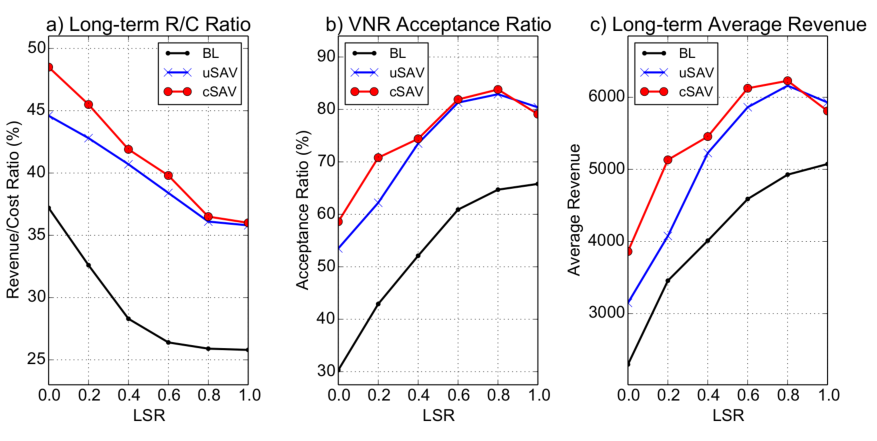
\includegraphics[width=1\textwidth]{perf_algo2.pdf}\newline
	\caption{\label{graph12} Testresultate mit variabler LSR für Kosten/Nutzen, Akzeptanz und Durchschnitts-Nutzen (beginnend links). \cite{algo2}}
\end{center}
\end{figure}

Man sieht in Abbildung~\ref{graph12} die drei, am schwersten gewichteten Aspekte dieses Ansatzes. Der Kosten-/Nutzen-Wert sinkt mit zunehmender LSR, während die Akzeptanz und der Nutzen gegenteiliges Verhalten zeigen. Die vorhandenen Laufzeitanalysen der Algorithmen bestätigen die Aussagen der Authoren. uSAV führt hier mit Werten zwischen 6 und 10 Minuten, während cSAV erst nach 14 bis 25 Minuten brauchbare Ergebnisse liefert. Hinzuzufügen sei hier, dass für alle Simulationen der einfachste Sicherheitsvektor verwendet wurde und bei Verwendung eines ausgeprägten Vektors die Rechenzeit mit Sicherheit andere Maße annimmt.


\subsection{Vergleich der beiden Ansätze}
\label{subsec:svne_vergleich}

Um nun die beiden vorgestellten Ansätze in einen Vergleich zu bringen, möchten wir uns hier nicht auf die Ergebnisse der Testszenarien konzentrieren, sondern auf die unterschiedlichen Herangehensweisen.

Der - für diese Arbeit wichtigste - Unterschied zwischen den beiden Ansätzen bezieht sich auf Granularität der Sicherheitsanforderungen. Ansatz 1 versucht hier mittels drei, auf Teilelemente bezogene, Sicherheitspläne Schutz zu bieten. Ein Vorteil dieses Vorgehens liegt klar in der Einfachheit der Umsetzungsmöglichkeit. Die Sicherheitsoptionen sind leicht verständlich und bieten eine gute Grundlage für die Abbildung sicherer Systeme. Nachteile könnten sich aus der Starrheit des Sicherheitssystems und dem Kostenfaktor ergeben. Mit Starrheit des Sicherheitssystems ist die Vernachlässigung vieler Sicherheitsaspekte und die ausschließliche Fokussierung auf die Isolation der Komponenten gemeint. Zwar bietet die Isolation eines gesamten Netzbereichs einen gewissen Schutz, eine Komprommittierung des physischen Hosts durch die isolierte VM ist so jedoch nicht gänzlich ausgeschlossen, was die Sinnhaftigkeit der teuren Netz-Isolation wiederum in Frage stellt. Der Kostenfaktor betrifft den Resourcenverbrauch bei High-Security-VNR. Man stelle sich ein Szenario vor, indem jeder VNR auf High-Security-Abbildung besteht. Virtualisierung wäre in diesem Szenario hinsichtlich der Resourcen-Optimierung völlig überflüssig. Ansatz 2 bietet hier etwas mehr Flexibilität sowie Präzision. Durch eine sinnvolle Definition der Sicherheitsvektoren könnte hier jeder mögliche Angriffsvektor benannt und die zugehörige Sicherheitsstufe bestimmt werden. Sollten neue Verwundbarkeiten entdeckt werden, könnten auch diese durch Hinzufügen entsprechender Werte zum Vektor binnen kurzer Zeit und mit wenig Aufwand integriert werden. Zusätzlich bietet das Zusammenspiel von Anforderungs- und Sicherheits-Level eine gewisse Flexibilität bezüglich der Resourcennutzung. 

Abhängig vom Einsatzzweck sind dahingehend beide Ansätze als sinnvoll zu betrachten. Ansatz 1 eignet sich für Situationen, in denen optimale Resourcennutzung weniger im Mittelpunkt steht als Flexibilität bezüglich Simulation von Hardware-Elementen. In der Mobilkommunikation beispielsweise sind Anbieter von dedizierter Hardware abhängig. Sollte hier der Schritt zur Virtualisierung gewagt werden, sind die Betreiber der Systeme für die Sicherheitseinstellungen der physischen sowie auch der virtuellen Hosts selbst zuständig. Ein High-Security-VNR für die Abbildung der zu simulierenden Geräte bietet also eine ausreichende Grundlage. Alle weiteren Sicherheitsmechanismen sind selbst zu wählen und benötigen keine Übereinkunft/Absprache zwischen mehreren Parteien (bspw. Inp und SP). Ansatz 2 ist für Szenarien geeignet in denen InP und SP zwei verschiedene Parteien sind und optimale Resourcennutzung für den InP eine große Rolle spielt. Nach ausreichender Definition der Sicherheitsvektoren, ist eine Übereinkunft bezüglich der Sicherheitsmechanismen unproblematisch. Wichtig ist hierbei jedoch die Überprüfung der Einhaltung der Sicherheitsbestimmungen seitens des SP, um den Schutz der gesamten Infrastruktur zu gewährleisten. Ein weiterer positiver Aspekt hierbei ist die Möglichkeit seitens InP an den SP Mindestanforderungen zu stellen.

Ein anderer Unterschied zwischen den beiden Ansätzen ist die Herangehensweise bei der Berechnung. Pre-Processing kann das Abbilden der VNR deutlich verkürzen, muss jedoch sequenziell durchgeführt werden und benötigt bei komplexeren VNR vermutlich auch eine nicht zu vernachlässigende Inanspruchnahme von Rechenzeit. Ansatz 2 versucht an dieser Stelle mittels Heuristiken und zweier unterschiedlicher, unter Umständen parallel laufender Algorithmen das gewünschte Ziel zu erreichen. Inwiefern welcher der beiden Ansätze bezüglich der Berechnungszeit als Gewinner hervorgeht, lässt sich aufgrund der unterschiedlichen Testsimulationen zu diesem Zeitpunkt nicht bestimmen. Eine Online-Evaluation beider Algorithmen zu selben Bedingungen würde hier Abhilfe schaffen.


\section{Schlussfolgerung und Ausblick}
\label{sec:schluss}

Das Ziel einer Klassifizierung von Sicherheitsrisiken und der Darstellung zweier SVNE-Algorithmen konnte in dieser Arbeit umgesetzt werden.

\dots

Die Komplexität des Themengebietes lässt hier keine Angabe einer Richtung zukünftiger Entwicklungen zu. Die Herangehensweise von VNR-Algorithmen sollte sich stets an die Bedürfnisse der Einsatzzwecke anpassen und da Virtualisierung den Einsatzzwecken kaum Grenzen in den Weg stellt, wird es wohl auch in Zukunft eine Vielzahl verschiedener Algorithmen mit unterschiedlichen Hauptaspekten geben. Die hier gezeigten Algorithmen sind nur zwei von vielen und sollen die Verschiedenartigkeit der möglichen Herangehensweisen verdeutlichen. Eine Verwendung neuronaler Netze oder anderen KI-Elementen wie Machine-Learning ist hierbei nicht auszuschließen.


%Frage: Auf welcher Ebene wird virtualisiert? Auf IP-Ebene? Was ist dann aber mit IP-Support-Protokollen (ARP)? Oder nicht-IP-Protokollen? Will ich ein Netzwerk virtualisieren, oder nur den IP-Verkehr? Verkapselung führt zu Leistungseinbußen. \cite{cabuk2007towards}







%Werke ins Literaturverzeichnis eintragen, die wichtige Grundlage für diese Arbeit waren, aber nicht direkt zitiert wurden:
\nocite{fischer2011position}

~\newpage
\bibliography{literatur}{}

\end{document}



